\newpage
\section*{Appendix}
The following section has been added to the appendix for the purposes of demonstrating modeling using PyGIMLi highlighting library usages. \textit{We do however acknowledge that raytracing for a layered model has an analytical solution where care is taken to account for direct and critically refracted waves (governed by Snell’s law), which here is taken as an approximation of the raypath that is found by finding the shortest-path through a grid of nodes.}
\section*{Modelling a Synthetic 2D Profile}

\begin{figure}[H]
\centering
\begin{minipage}[t]{0.48\textwidth}
    \centering
    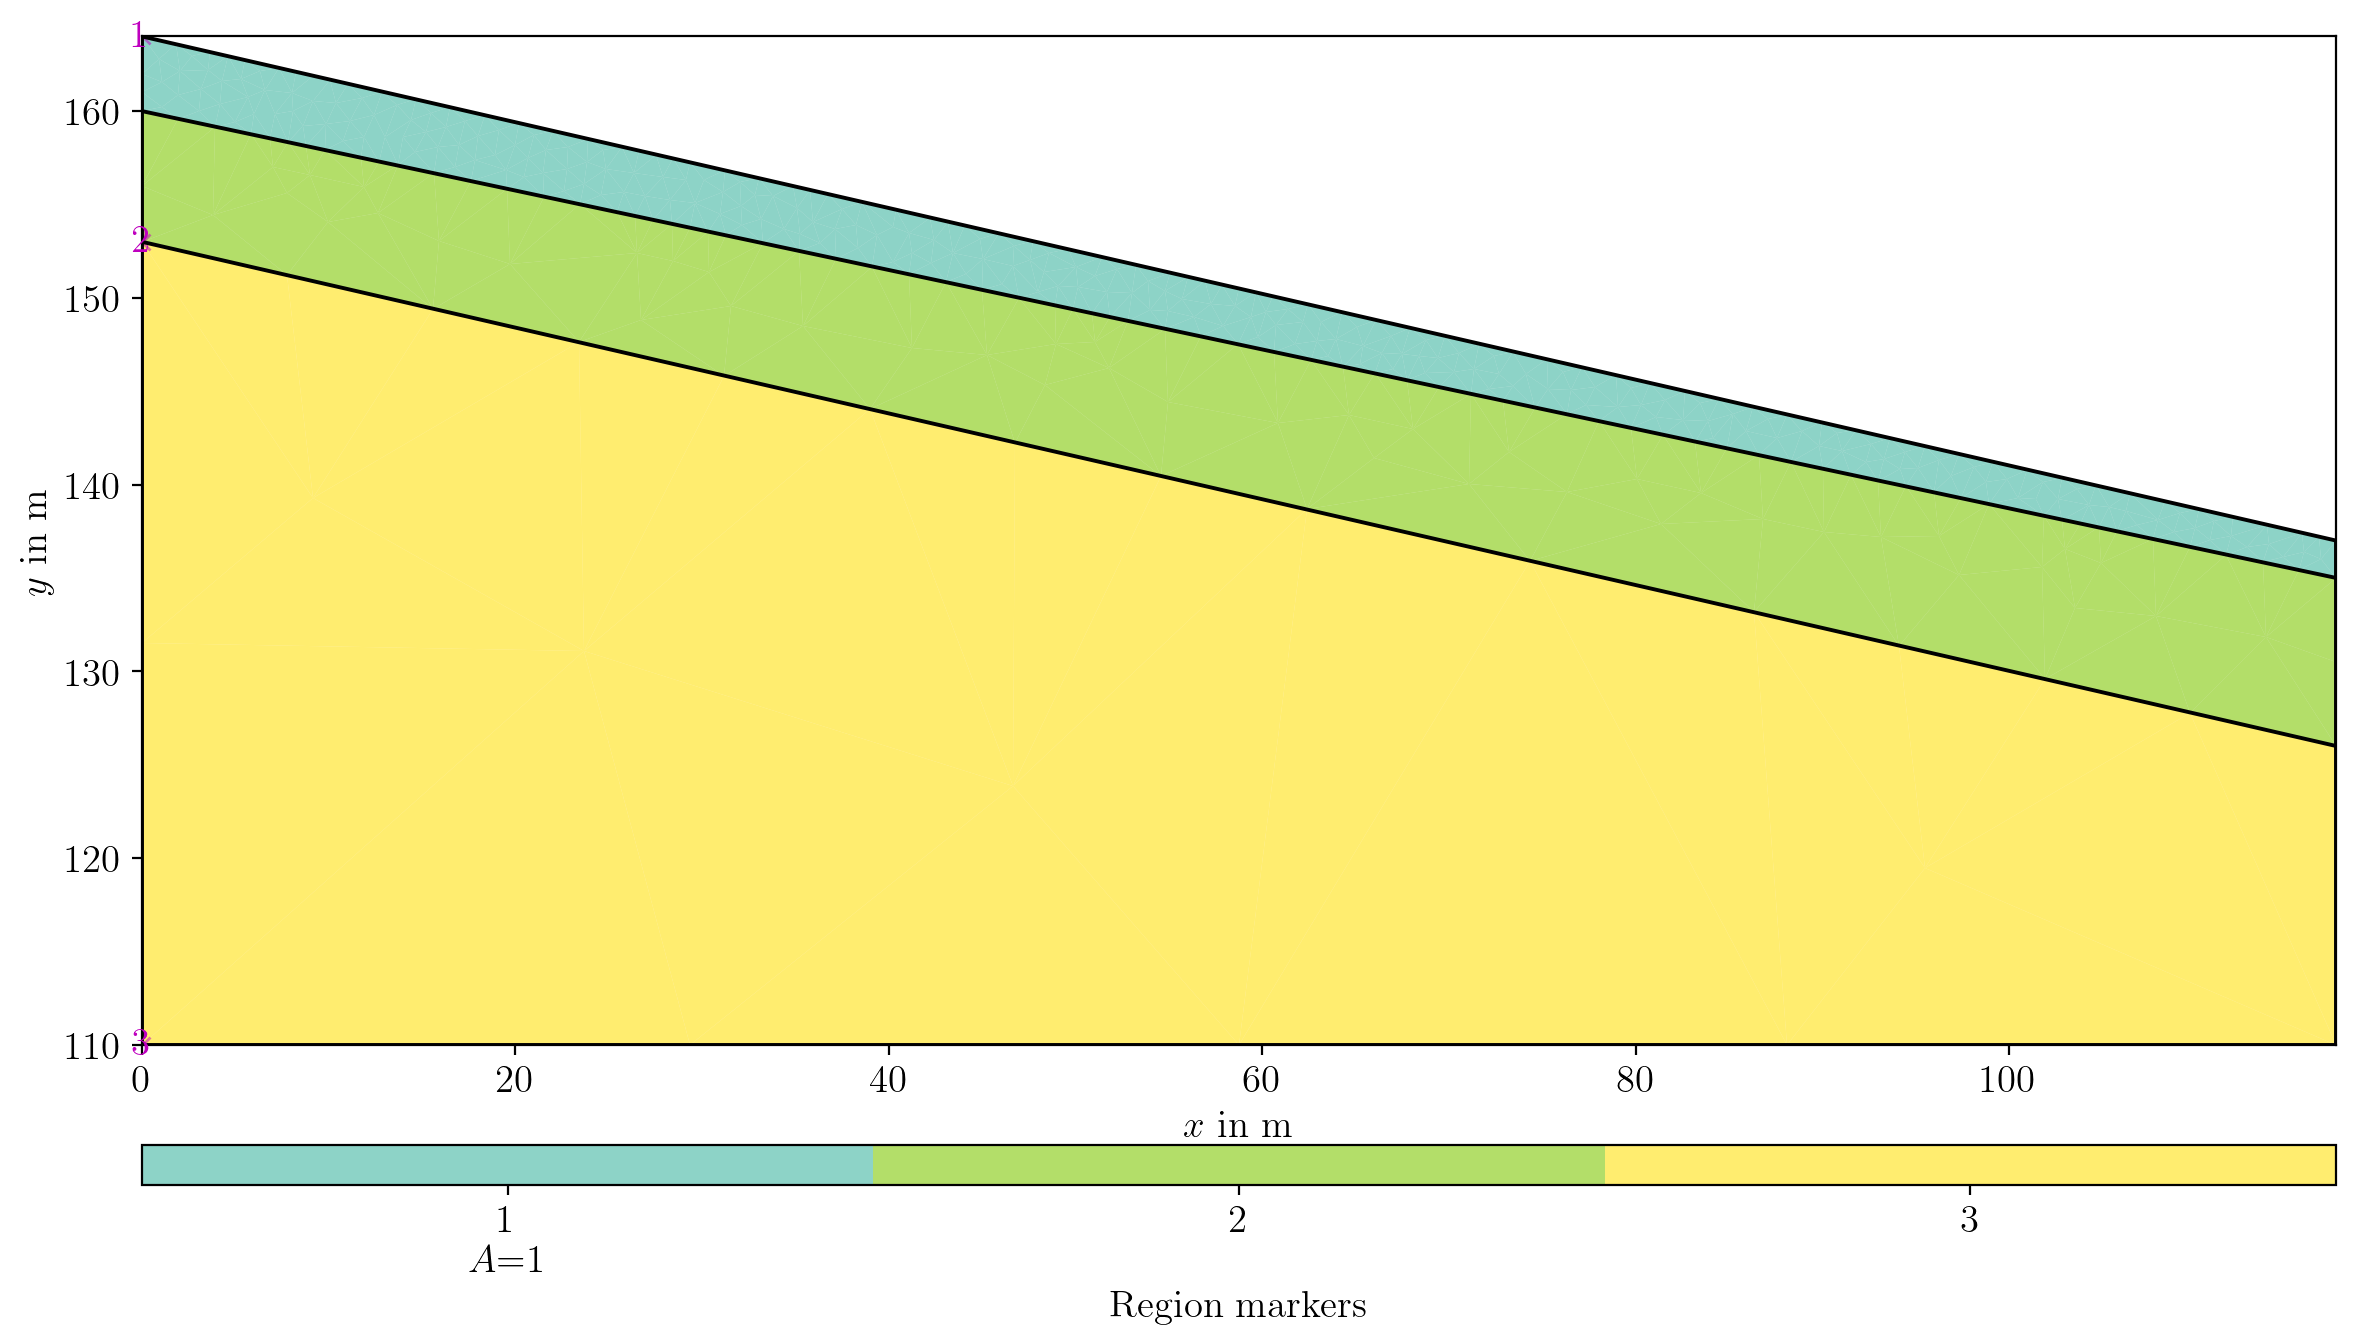
\includegraphics[width=\textwidth]{Media/p1/1.png}
\end{minipage}
\hfill
\begin{minipage}[t]{0.48\textwidth}
    \centering
    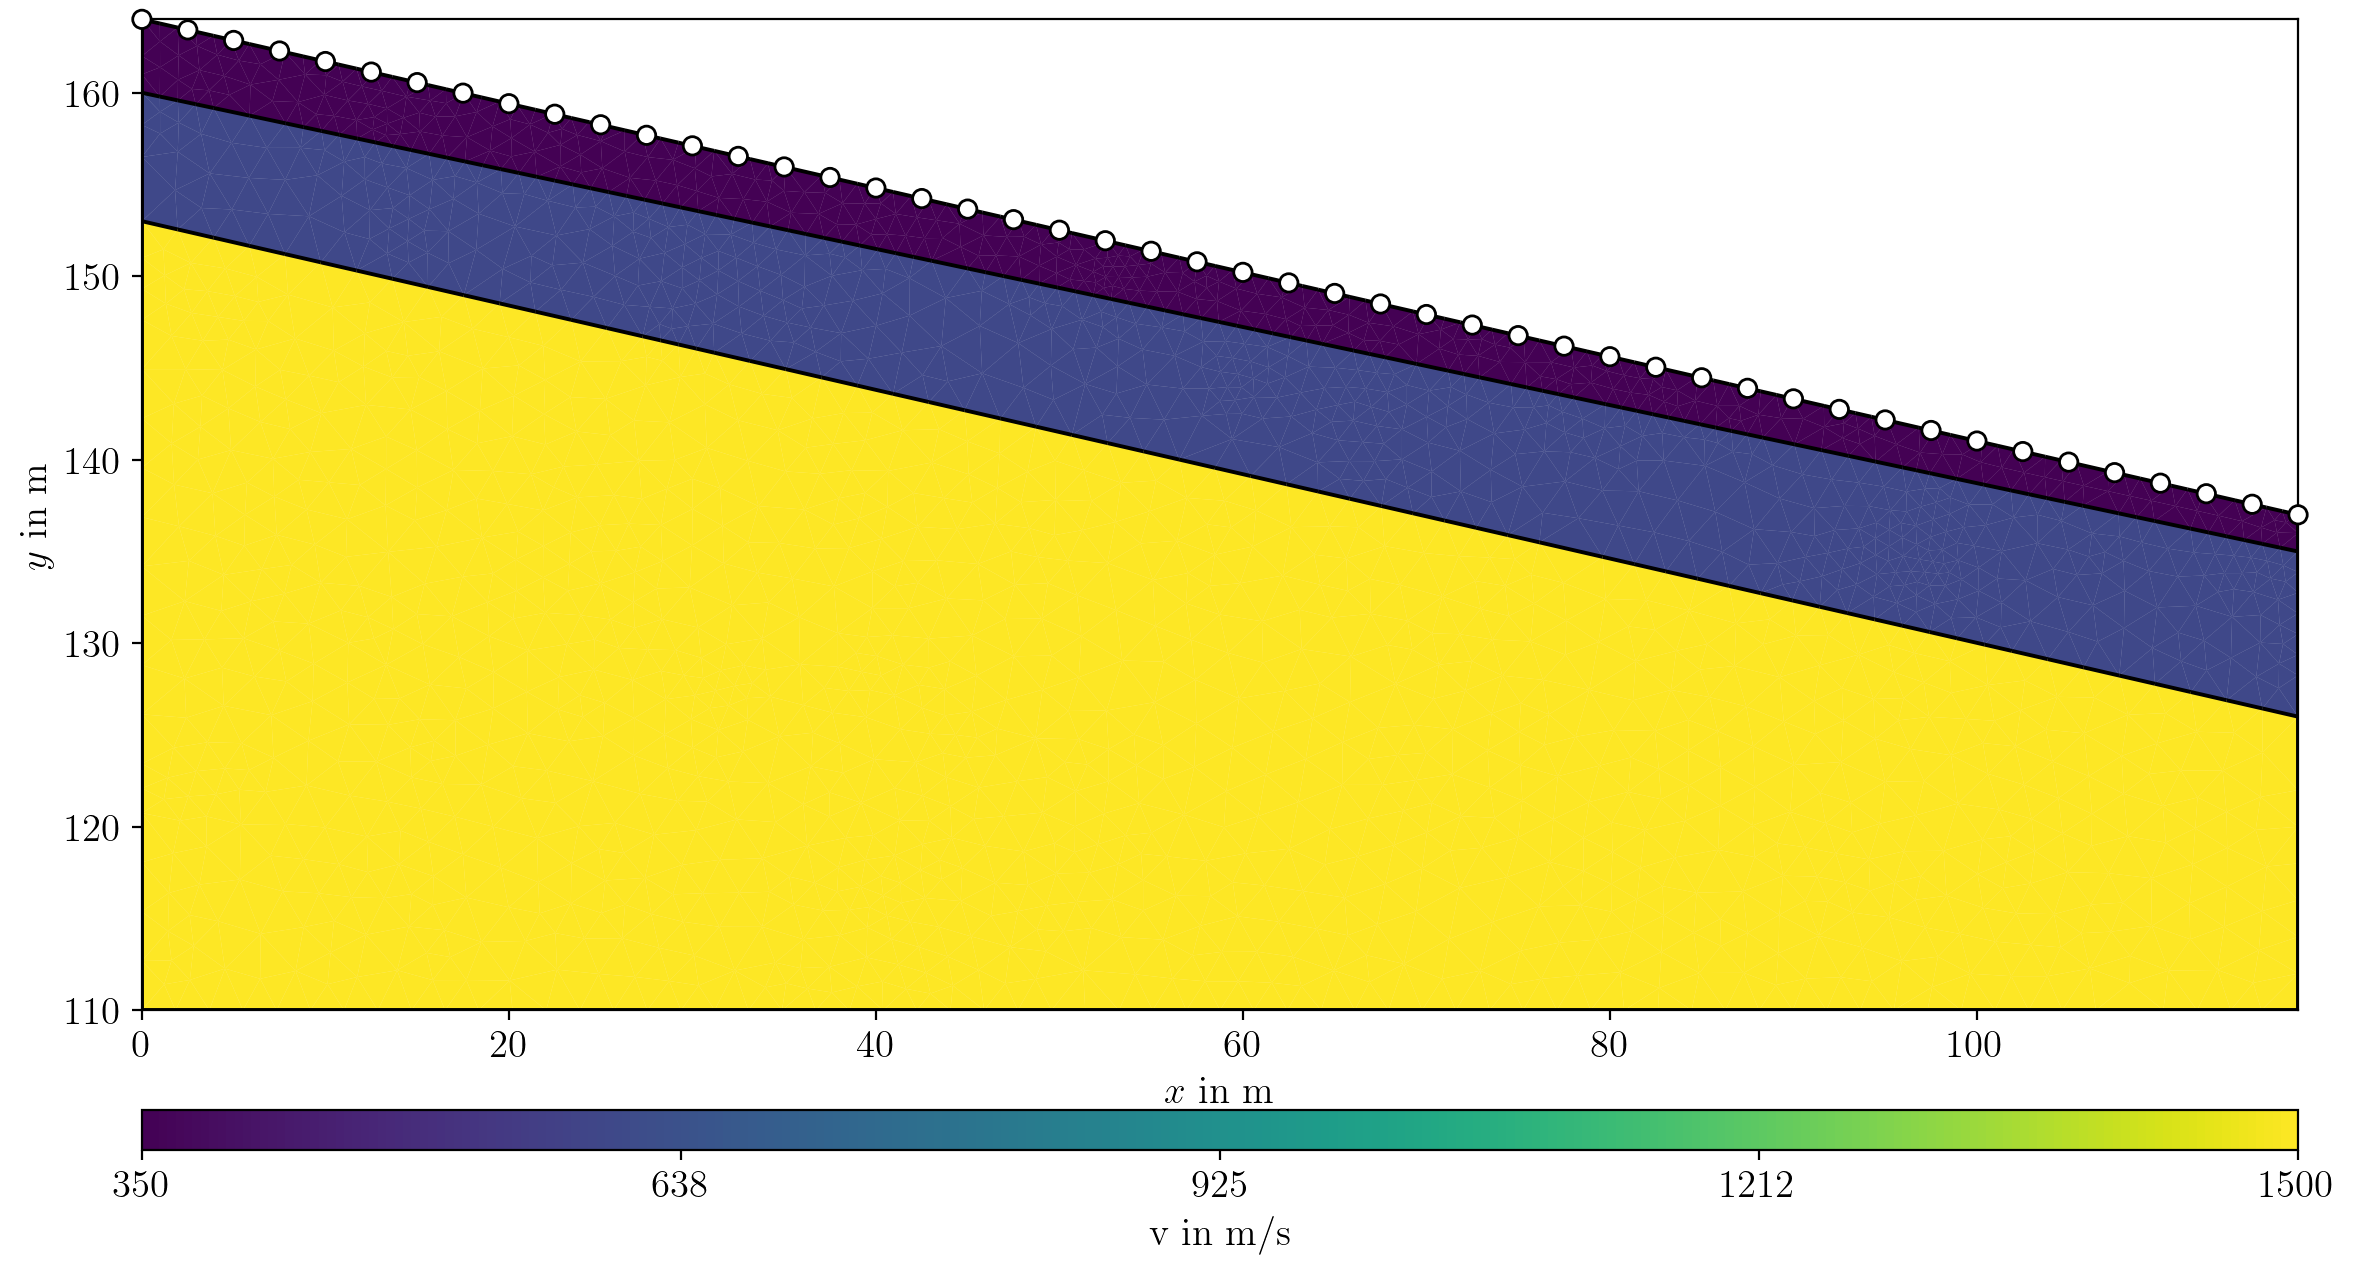
\includegraphics[width=\textwidth]{Media/p1/3.png}
\end{minipage}
\caption{(a.) Sloping Layered geometry (b.) Geophone and shot positions on the sloped surface. White circles indicate receiver positions, and source positions are at equivalent coordinates}
\end{figure}

\subsection*{Objective}
Recover a layered 2D velocity model from first-arrival (refraction) picks along a surface profile.

\subsection*{True model and parameterization}
\begin{itemize}
  \item Three-layer sloping model defined by polygons coordinates (m):
  \begin{verbatim}
layer1 = [[0.0,164], [117.5,137], [117.5,135], [0.0,160]]  (marker=1, v=350 m/s)
layer2 = [[0.0,153], [0.0,160], [117.5,135], [117.5,126]]  (marker=2, v=600 m/s)
layer3 = [[0.0,110], [0.0,153], [117.5,126], [117.5,110]]  (marker=3, v=1500 m/s)
  \end{verbatim}
    \item \textbf{Layer 1 (350 m/s)}: Unconsolidated sediments, weathered zone, or saturated clay
    \item \textbf{Layer 2 (600 m/s)}: Partially consolidated sediments or fractured rock
    \item \textbf{Layer 3 (1500 m/s)}: Consolidated bedrock, dense limestone, or crystalline basement
\end{itemize}

\subsection*{Geophone Deployment \& Shot Configuration}
A linear array of $N_{\text{geo}} = 48$ geophone stations is deployed along the topographic surface. The horizontal positions are uniformly distributed:

\begin{equation}
x_i = \frac{i}{N_{\text{geo}} - 1} \times 117.5 \, \text{m}, \quad i = 0, 1, \ldots, 47
\end{equation}
The vertical positions are adapted to follow the sloped surface:
\begin{equation}
y_i = m_s \cdot x_i + y_{\text{intercept}} = 0.23 \cdot x_i + 137
\end{equation}
Shots (seismic sources) are deployed with a fixed shot distance interval:
\begin{equation}
\Delta x_{\text{shot}} = 3 \, \text{m}
\end{equation}
This creates a reciprocal refraction dataset where shots and receivers occupy the same surface locations. The resulting measurement scheme consists of:
\begin{itemize}
    \item Total number of shots: $N_{\text{shots}} \approx 40$
    \item Total number of receivers per shot: $N_{\text{geo}} = 48$
    \item Total number of ray paths: $\approx 1920$
\end{itemize}

% \subsection*{Synthetic data generation (forward modelling)}
% \begin{itemize}
%   \item Forward simulation call:
%   \texttt{tt.simulate(slowness=1.0/vp, scheme=scheme, mesh=mesh, noiseLevel=0.001, noiseAbs=0.001, seed=1337)}.
%   \item Noise: relative noise = 0.1\% (\texttt{noiseLevel=0.001}), absolute noise = 0.001 s, seed fixed for reproducibility.
% \end{itemize}

% \subsubsection*{Dijkstra Ray-Tracing Operator}

% PyGIMLi creates a \textbf{TravelTimeDijkstraModelling} forward operator takes a velocity model $\mathbf{m}$, converts velocity to slowness: $s = 1/v$, traces rays from each shot to each receiver using Dijkstra's algorithm, returns predicted travel times $\mathbf{d}_{\text{pred}} = \mathbf{f}(\mathbf{m})$

% \subsubsection*{How Dijkstra Ray Tracing Works}
% Dijkstra's algorithm solves the \textbf{eikonal equation} numerically:
% \begin{equation}
% |\nabla T(\mathbf{r})|^2 = \frac{1}{v^2(\mathbf{r})}
% \end{equation}
% \textbf{Algorithm steps}:
% \begin{enumerate}
%     \item Initialize travel-time field $T$ to infinity everywhere except at the source: $T(\text{source}) = 0$
%     \item Build a directed graph where:
%     \begin{itemize}
%         \item Nodes = mesh vertices
%         \item Edges connect adjacent nodes
%         \item Edge weight = distance $/ v_{\text{avg}}$ (slowness-weighted distance)
%     \end{itemize}
%     \item Use Dijkstra's shortest-path algorithm to compute minimum travel times to all receivers
% \end{enumerate}

% \textbf{Computational complexity}: $O(n \log n)$ where $n$ is the number of mesh nodes

\subsection*{First-break Travel Times}
Each colored curve corresponds to a different shot location along the survey line, and the horizontal axis shows the position of geophones (receivers) in meters. The vertical axis records the measured arrival (first-break) travel times in seconds for each shot-receiver pair.
\begin{itemize}
    \item \textbf{X-Axis} (\texttt{x (m)}): Geophone position along the survey line on the surface.
    \item \textbf{Y-Axis} (\texttt{Traveltime (s)}): Recorded time for the first seismic arrival at each receiver, with time increasing downward.
    \item \textbf{Multiple Curves/Colors}: Each colored line traces first-arrival times for a different shot position; the colors distinguish between different shots (sources).
    \item \textbf{Crossover Point}: The inflection or bend in each curve marks the transition from direct arrivals to refracted arrivals—a key diagnostic for determining subsurface velocities and layer depths.
\end{itemize}

\begin{figure}[H]
\centering
\begin{minipage}[t]{0.48\textwidth}
    \centering
    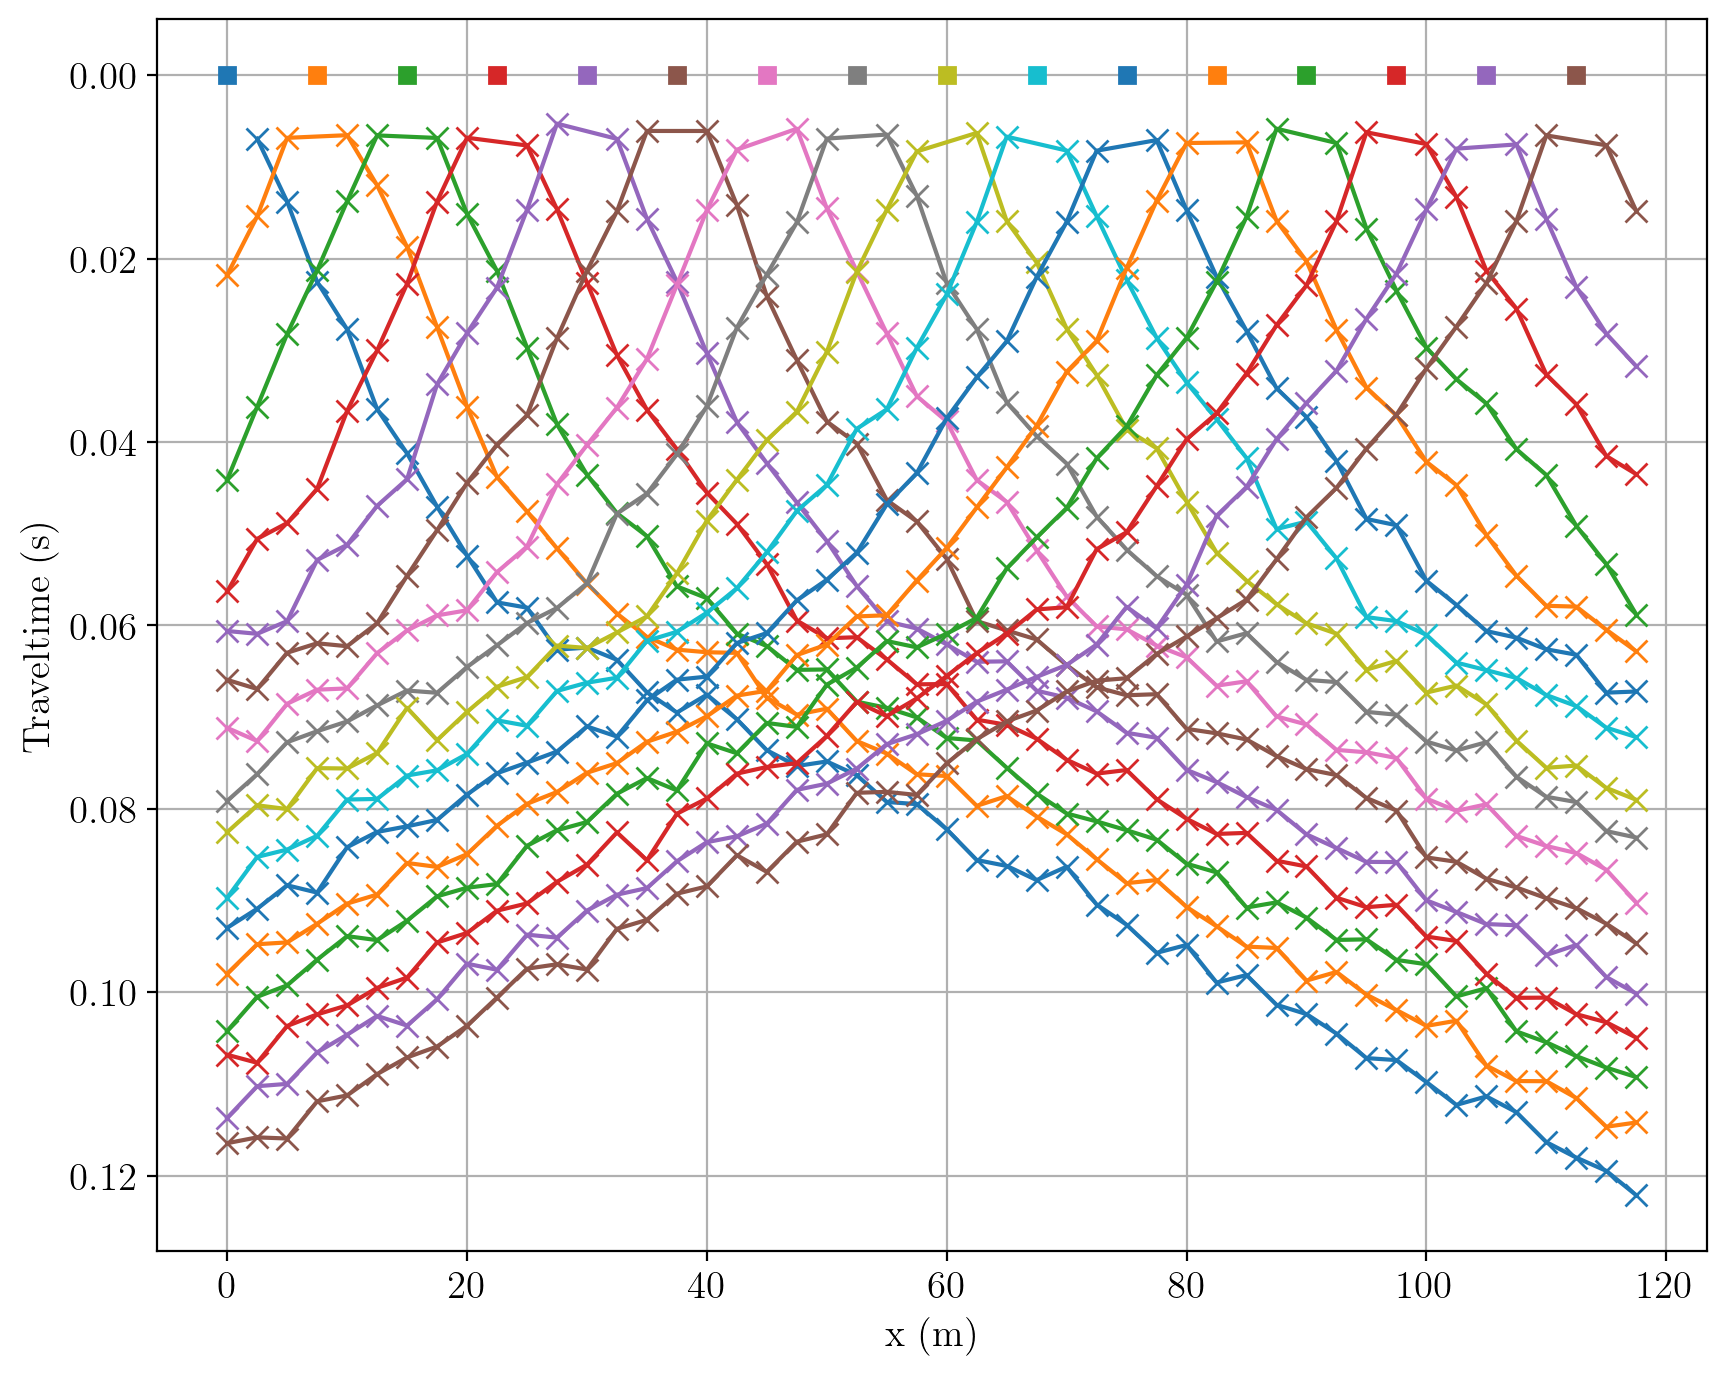
\includegraphics[width=\textwidth]{Media/p1/4.png}
\end{minipage}
\hfill
\begin{minipage}[t]{0.48\textwidth}
    \centering
    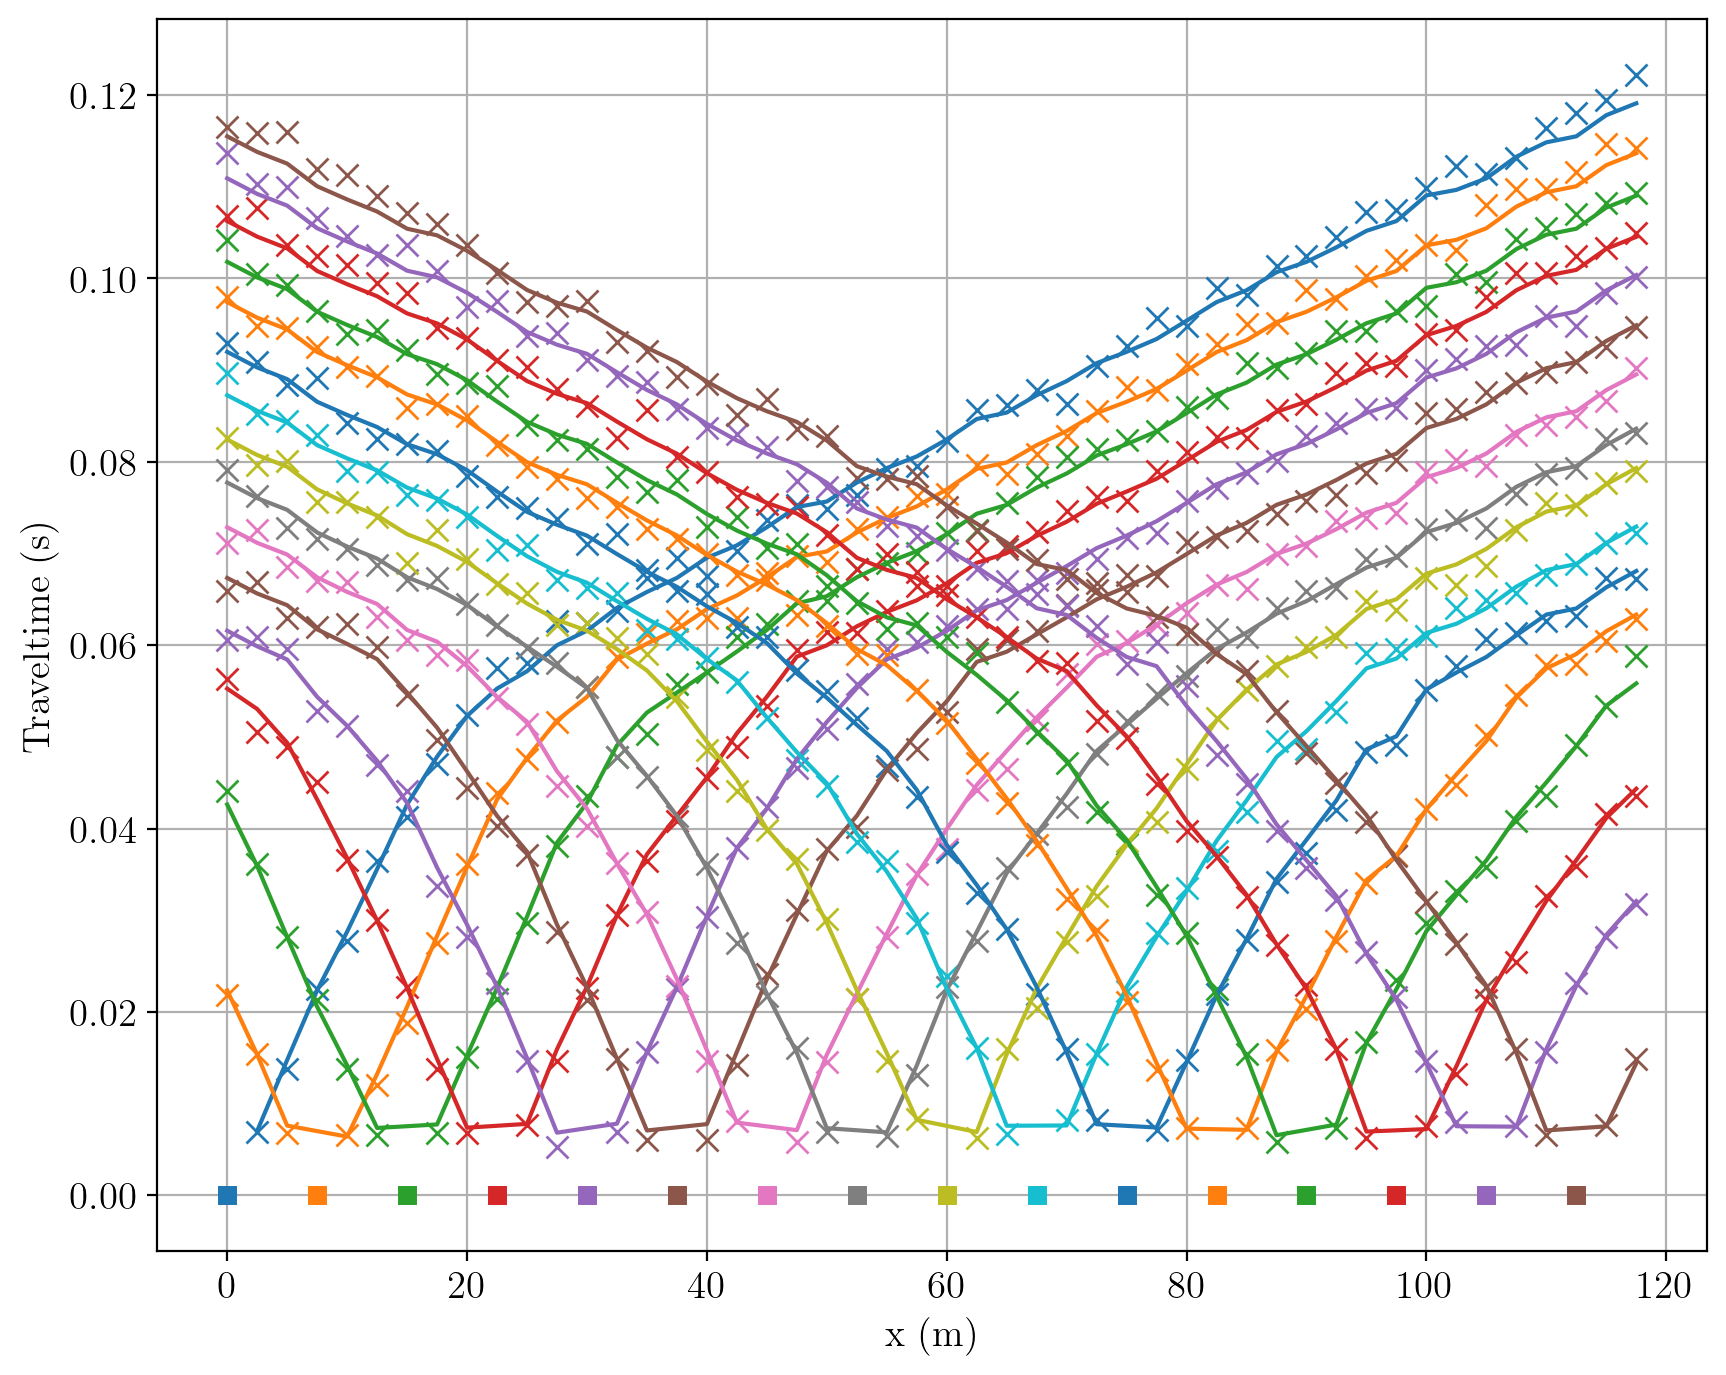
\includegraphics[width=\textwidth]{Media/p1/6.png}
\end{minipage}
\caption{(a.) Synthetic travel-time data simulated through the forward velocity model. The figure shows the first-break arrival times (in milliseconds) organized by shot-receiver pairs using a refraction tomography acquisition geometry. The squares represent the shot positions and the crosses represent the corresponding x location of geophone. (b.) The corresponding predicted arrivals calculated using the inverted velocity model through forward ray tracing indicating residual misfit.}
\end{figure}

\subsection*{Inversion settings}
\begin{itemize}
  \item Manager: \texttt{mgr = tt.TravelTimeManager(data)}.
  \item Inversion call used:
  \texttt{mgr.invert(secNodes=2, paraMaxCellSize=15.0, maxIter=10, verbose=True)}.
  \item Transformation: data transform = Identity; model transform = Logarithmic transform.
  \item Regularization: example printed \texttt{lam: 20.0} and used chi-square stopping criterion (stops when $\chi^2\le1$).
\end{itemize}

\begin{figure}[H]
\centering
\begin{minipage}[t]{0.48\textwidth}
    \centering
    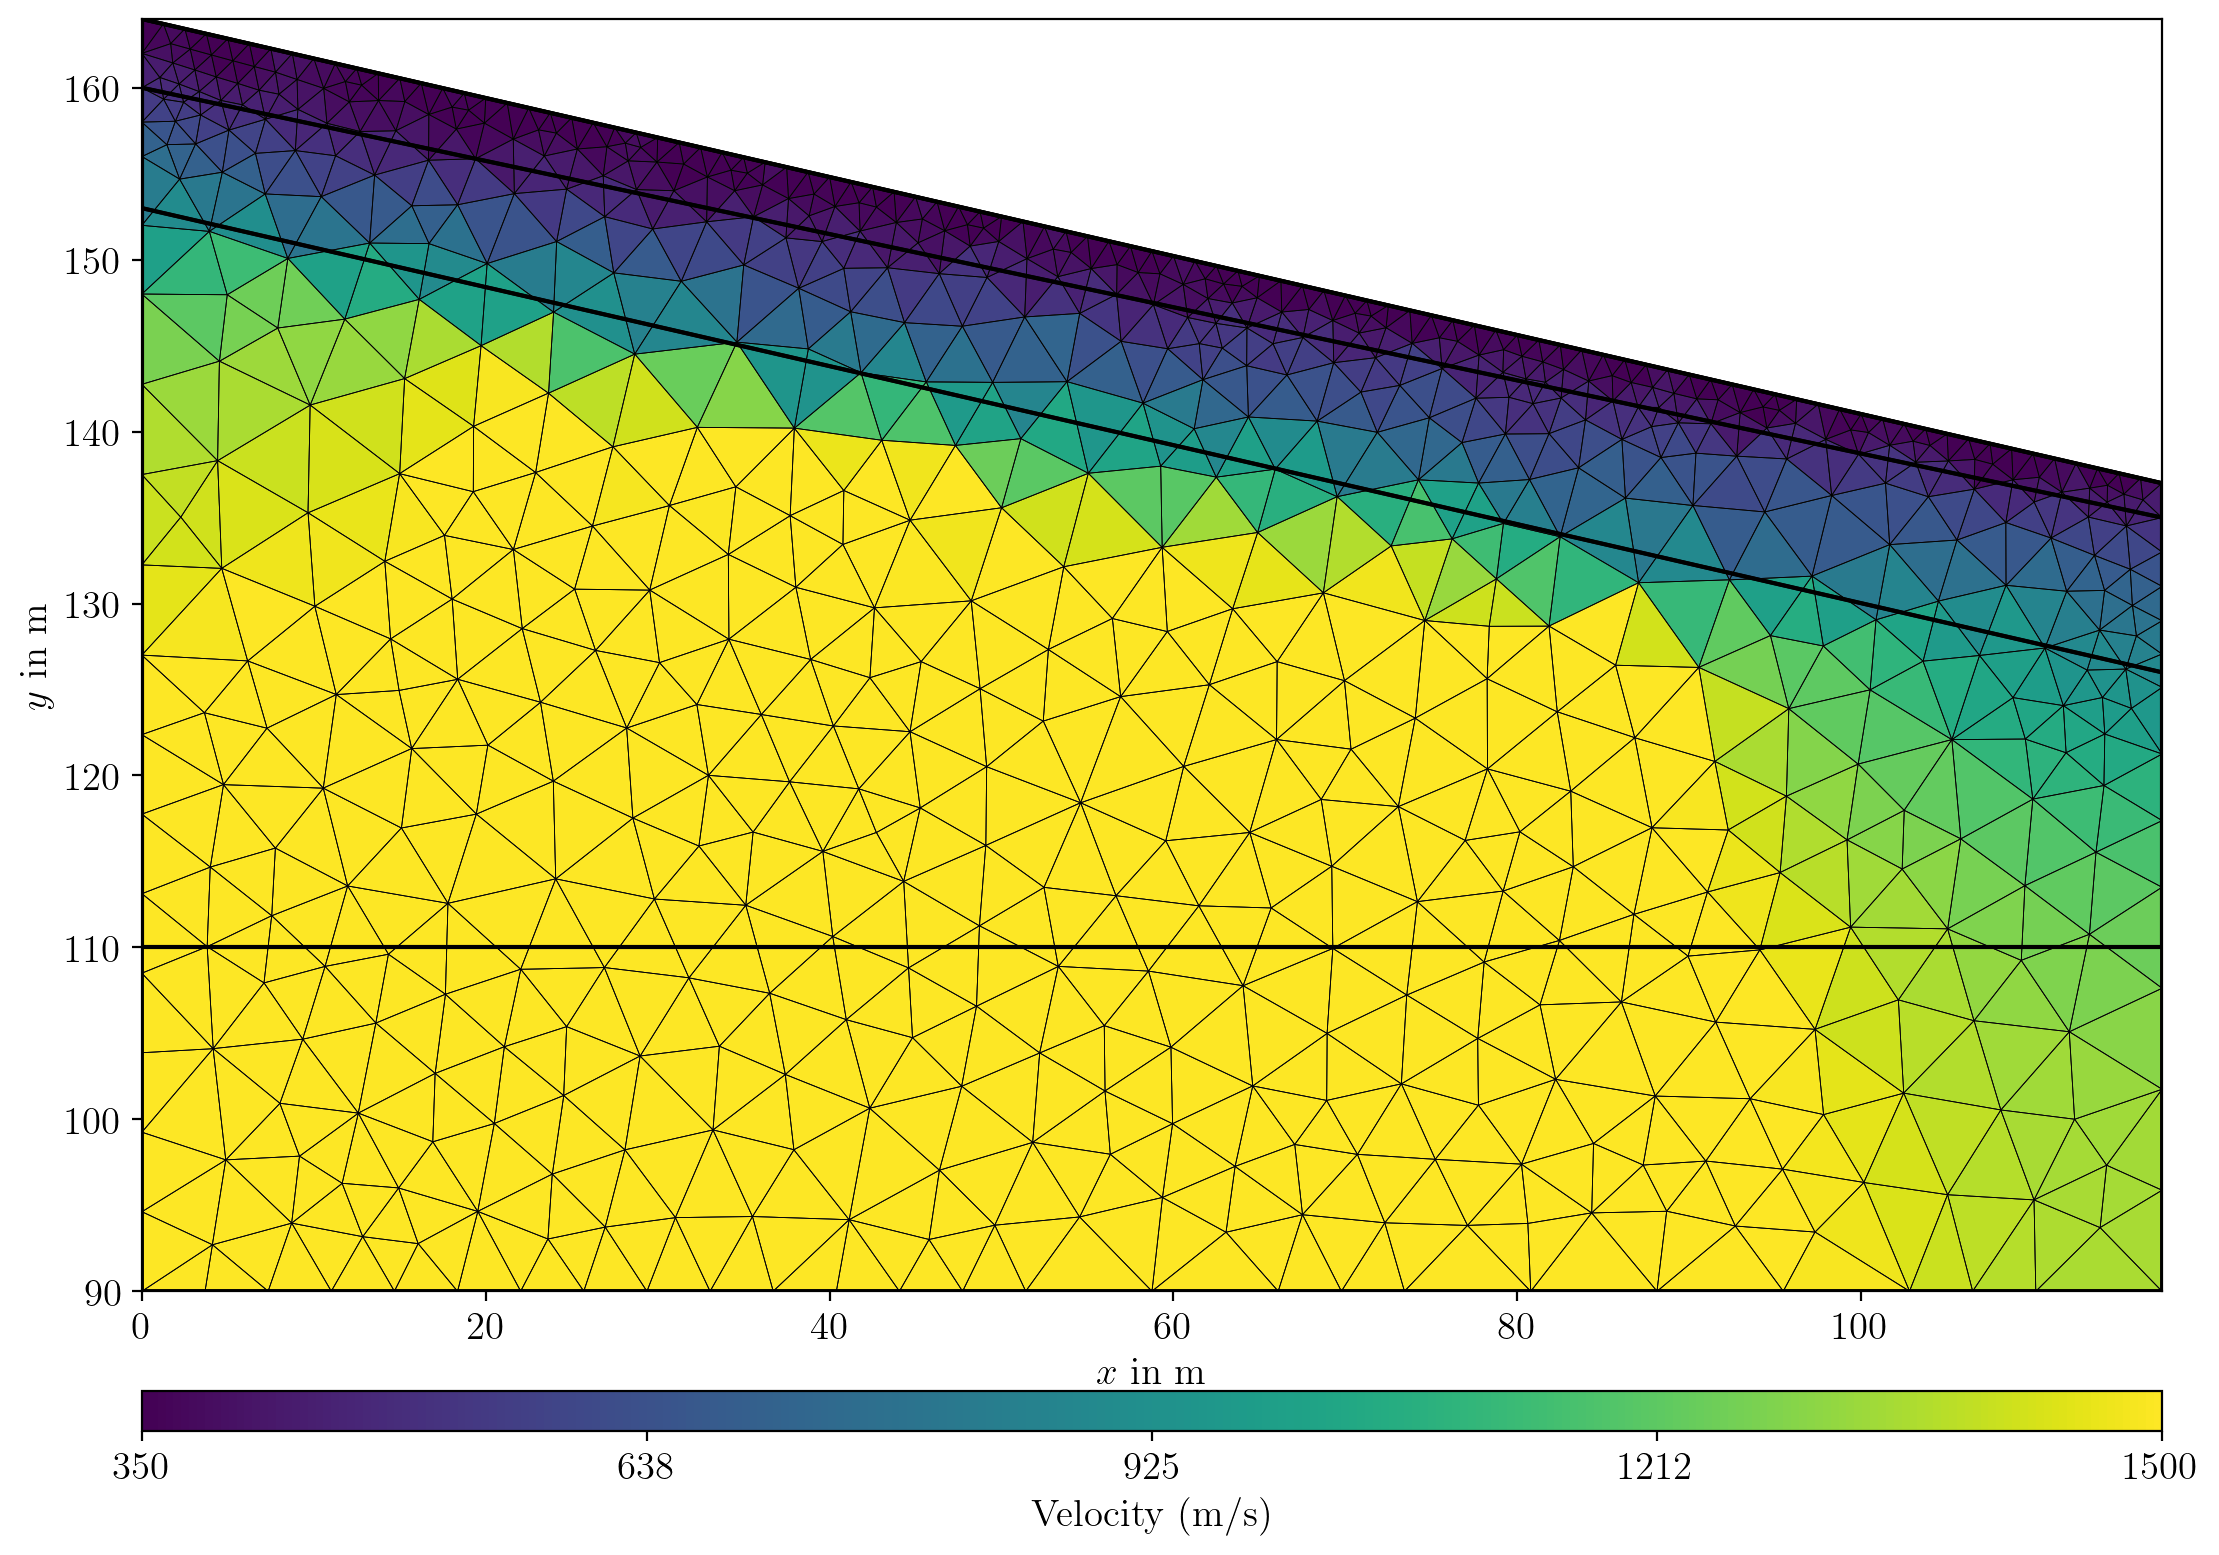
\includegraphics[width=\textwidth]{Media/p1/5.png}
\end{minipage}
\hfill
\begin{minipage}[t]{0.48\textwidth}
    \centering
    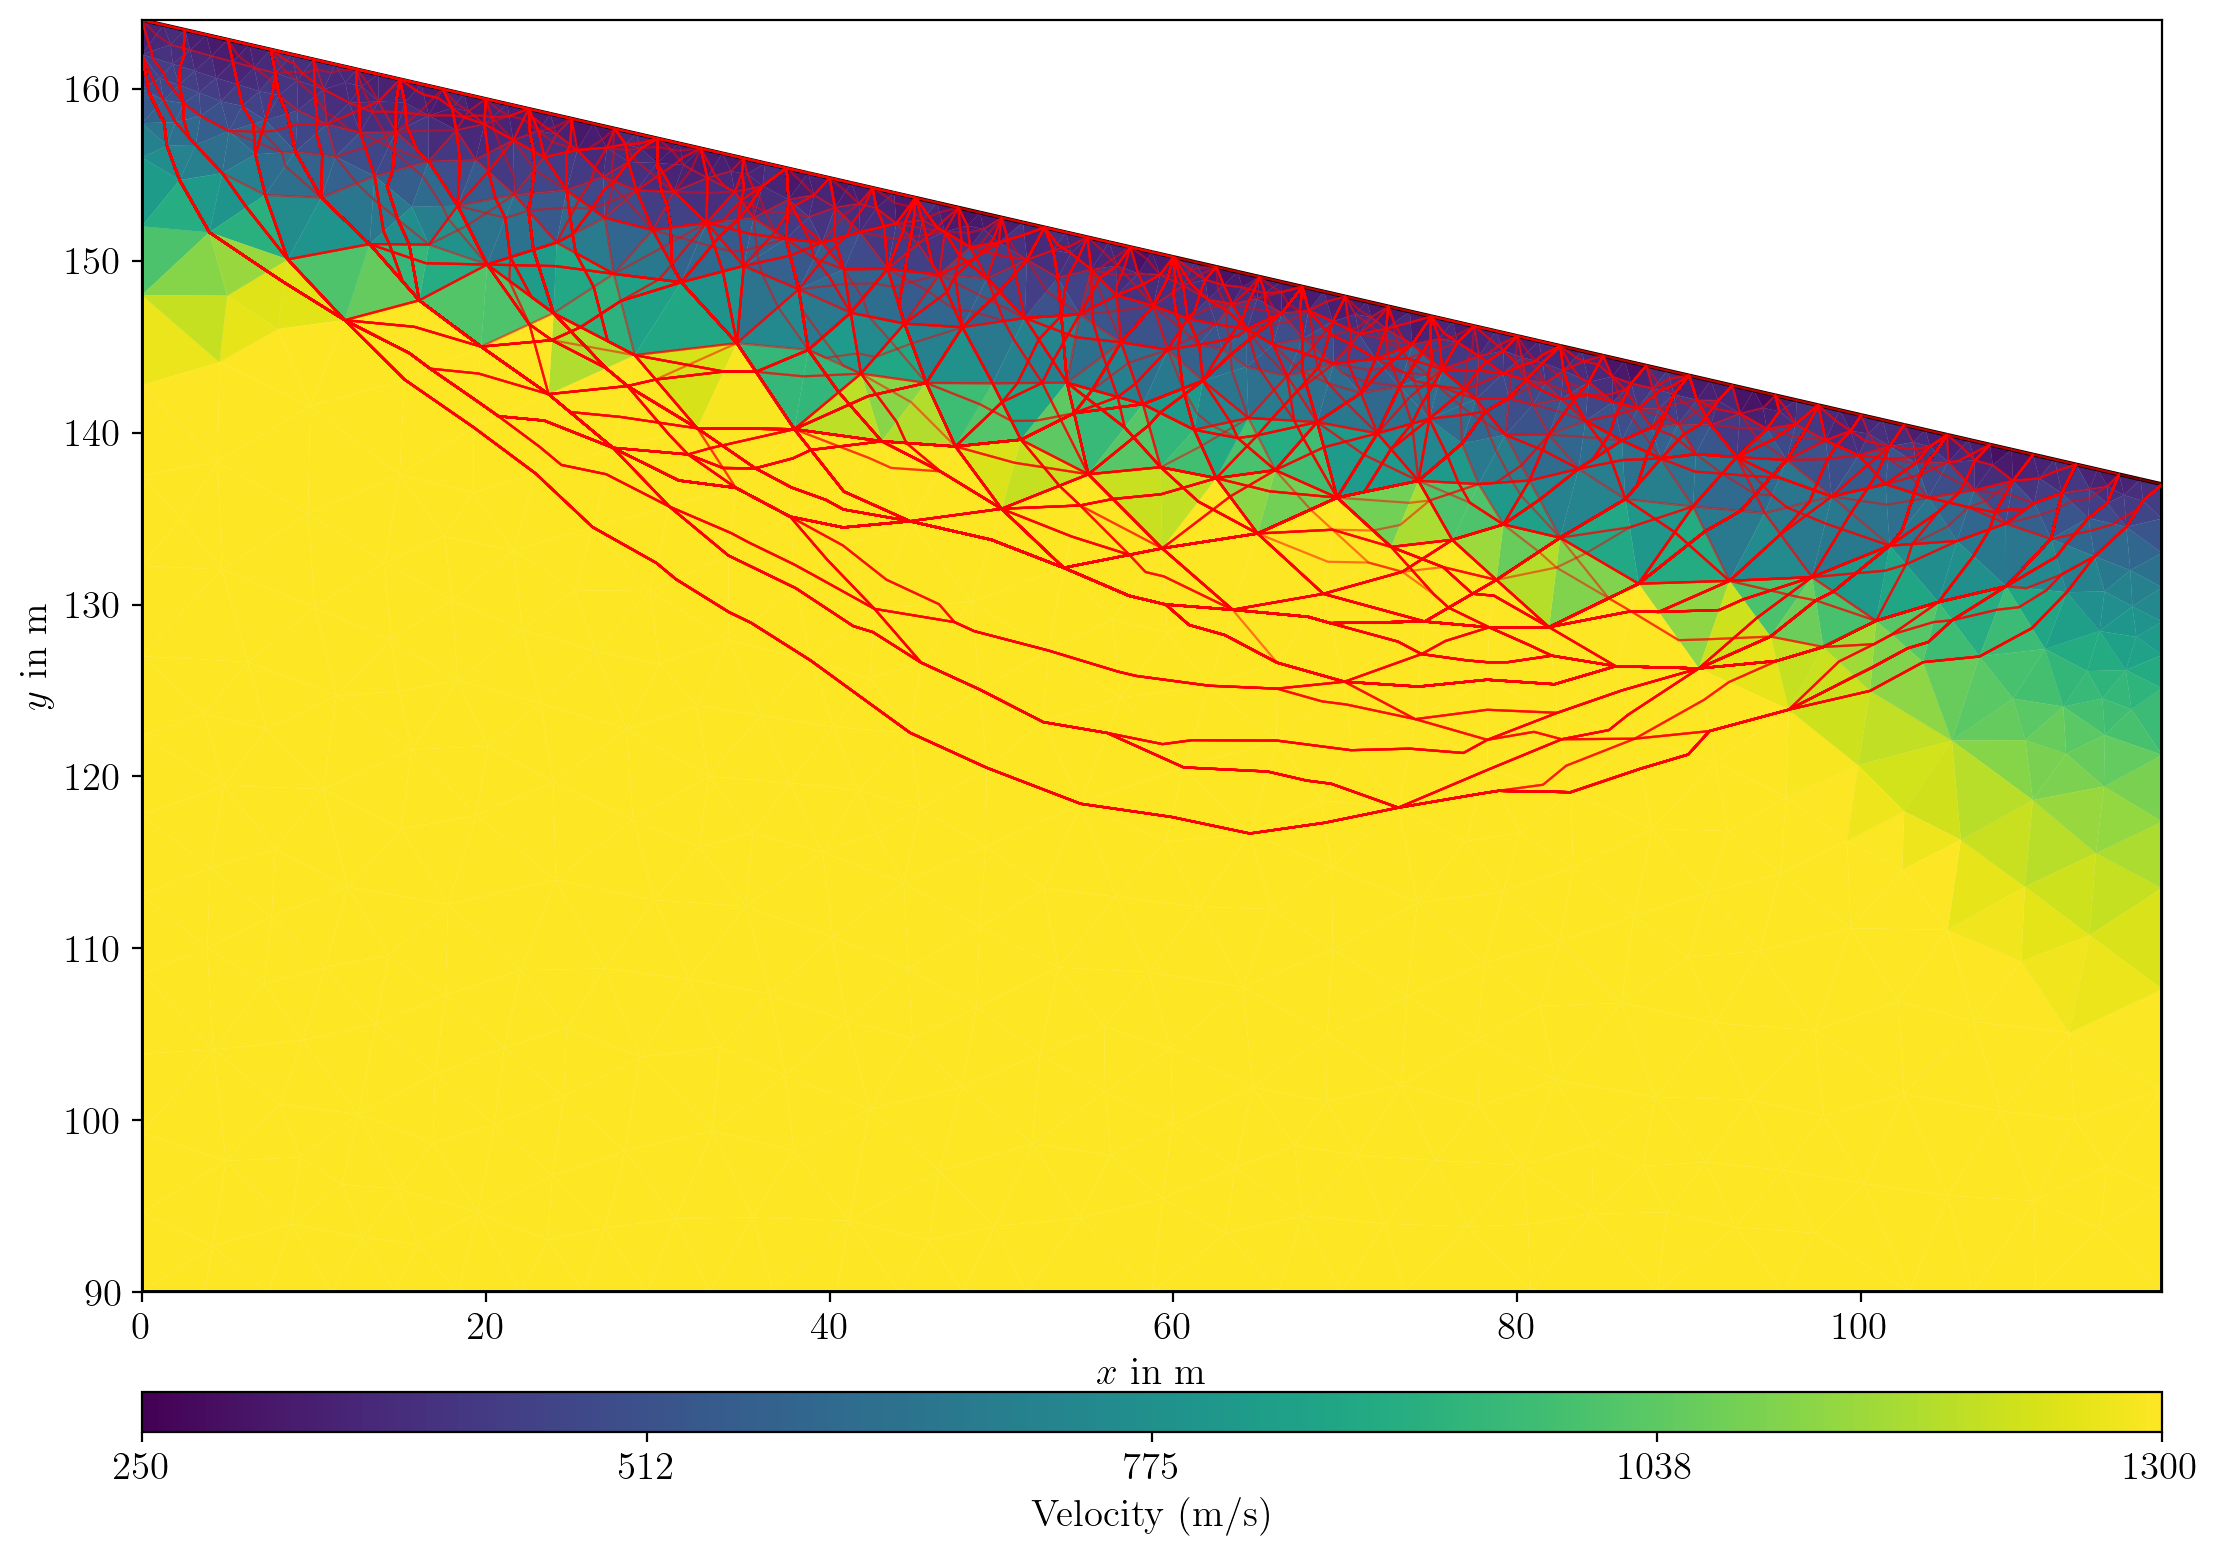
\includegraphics[width=\textwidth]{Media/p1/7.png}
\end{minipage}
\caption{(a.) Final inverted velocity model after convergence. Color indicates
velocity magnitude (b.) Ray paths computed through inversion. Different ray colors represent different shot-receiver pairs or ray-type categories. Refracted rays dominate the pattern, bending downward into faster velocity layers and returning to the surface. The ray coverage reveals illumination of all three layers across the model.}
\end{figure}
